\begin{figure}[!h]
\centering
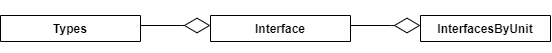
\includegraphics[scale=.8,]{Bilder/Quicktest/Klassen/KlasseAggregation.drawio.png}
\caption{Aggregation der Klassen}
\end{figure}
\begin{figure}[!h]
\centering
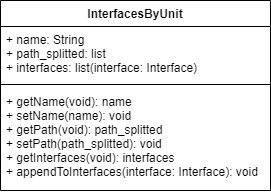
\includegraphics[scale=.9,]{Bilder/Quicktest/Klassen/KlasseInterfacesByUnit.drawio.png}
\caption{Klasse InterfacesByUnit}
\end{figure}
\begin{figure}[!h]
\centering
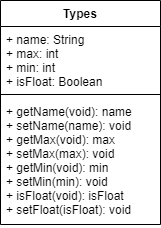
\includegraphics[scale=.9,]{Bilder/Quicktest/Klassen/KlasseType.drawio.png}
\caption{Klasse Type}
\end{figure}
\begin{figure}[!h]
\centering
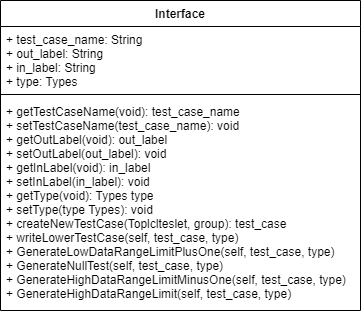
\includegraphics[scale=.9,]{Bilder/Quicktest/Klassen/KlasseInterface.drawio.png}
\caption{Klasse Interface}
\end{figure}